\chapter{Injection beam loss monitoring system}\label{sec:Injection bea loss monitoring system}

\section{Required performance}

At the SuperKEKB accelerator, the beam revolution period is approximately 10 us. Therefore, high time resolution is required to measure injection beam loss on a turn-by-turn basis. In addition, the sensors installed near the collimators are connected to readout boards via cables several hundreds meters long, resulting in signal attenuation. Thus, a sufficient high signal gain is required. Furthermore, the sensors have mo Sensor ust be radiation tolerant because the regions around the collimators are exposed to high radiation levels. 


\section{CLAWS sensor}
The CLAWS consists of a plastic scintillator and silicon photomultiplier (SiPM) \cite{Windel:2021zqa}. The scintillator serves as an active material and pruduce scintillator photons when traversed by charged particles. It has $30 \times30 \times 3 mm^3$ cube-shaped and central recess to accommodate the SiPM, which detects scintillator photons. 
The scintillator is wrapped in reflective foil to increases the number of photons detected by the SiPM. The reflective foil is covered with black tape to suppress the detection of unwanted ambient light.

The CLAWS sensors were originally developed to monitor radiation levels in the interaction region (IR) and provide input to the beam-abort system. More recently, CLAWS sensors have been installed near the collimators for the beam-abort system. The sensors have a time resolution of O(10 ns) and a gain of $10^5-10^6$, which are sufficient for measuring injection beam loss turn-by-turn. Since the radiation levels at the IR are significantly higher than those along the beam line, the sensor has demonstrated sufficient radiation tolerance for this application.

\begin{figure}
    \centering
    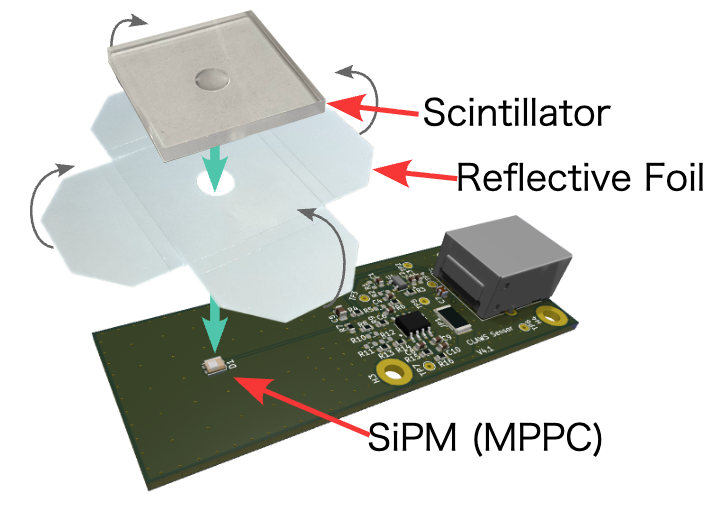
\includegraphics[width=0.8\columnwidth]{Figures/C04_Monitoring_system/CLAWS02.png}
    \caption{CLAWS sensor}
    \label{fig:CLAWS}
\end{figure}

\begin{figure}
    \centering
    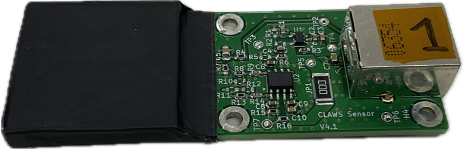
\includegraphics[width=0.6\columnwidth]{Figures/C04_Monitoring_system/CLAWS01.png}
    \caption{CLAWS sensor}
    \label{fig:CLAWS}
\end{figure}

\section{Install position}

(Overview of the collimator system and geometry is described in the previous chapter)

The previous loss monitor observed long-lasting injection beam loss at the vertical collimators. To monitor these losses in more detail, CLAWS sensors are installed at all vertical collimators and several horizontal collimators.  

\begin{table}[htbp]
    \centering
    \caption{Collimators equipped with CLAWS sensors in the LER and HER.}
    \label{tab:claws_collimators}
    \begin{tabular}{ll}
        \toprule
        \multicolumn{2}{c}{LER} \\
        \cmidrule(lr){1-2}
        Type & Collimator name \\
        \midrule
        Vertical   & D2V1 \\
        Vertical   & D3V4 \\
        Vertical   & D5V1 \\
        Vertical   & D6V1 \\
        Horizontal & D6H3 \\
        \bottomrule
    \end{tabular}
    \hspace{1.5cm}
    \begin{tabular}{ll}
        \toprule
        \multicolumn{2}{c}{HER} \\
        \cmidrule(lr){1-2}
        Type & Collimator name \\
        \midrule
        Vertical   & D1V1  \\
        Vertical   & D9V1  \\
        Horizontal & D9H2  \\
        Vertical   & D9V3  \\
        Vertical   & D12V1 \\
        Vertical   & D12V2 \\
        Vertical   & D12V3 \\
        Vertical   & D12V4 \\
        \bottomrule
    \end{tabular}
\end{table}

\begin{figure}[htbp]
    \centering
    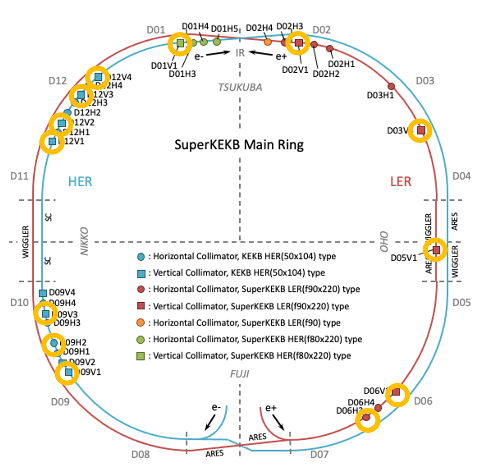
\includegraphics[width=1.0\columnwidth]{Figures/C04_Monitoring_system/mainring.png}
    \caption{Installed collimators}
    \label{fig:Installed collimators}
\end{figure}

The CLAWS sensors are mounted on support structure approximately 1m downstream of the collimators. Since radiation showers are expected to propagate parallel to the beam pipe, sensors were installed so that the elevation was as small as possible. 
\begin{figure}[htbp]
    \centering
    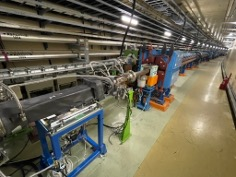
\includegraphics[width=0.8\columnwidth]{Figures/C04_Monitoring_system/install.png}
    \caption{CLAWS sensor install position}
    \label{fig:install_position}
\end{figure}


\section{Readout}

The CLAWS sigals are acquired synchronously with the 1 Hz prescaled injection kicker signal. The signals are transmitted through cables several hundreds meters long to the power supply buildings on the ground. Receiver boards installed in these buildings condition the signal before they are read by oscilloscopes. The oscilloscopes are controlled by PCs,  and waveform data covering 23 ms window after the trigger is acquired.

\section{Data correction, processing, recording}

The raw waveform data acquired oevr 23ms window consist of approximately 1 million samples, making it impractical to store all the raw data. Therefore, the following quantities are calculated from the raw waveforms and recorded instead: \\

\begin{enumerate}
    \item \textbf{Turn-by-turn beam loss:}
    The raw waveform is integrated over each turn after applying a threshold to identify beam-loss signals.

    \item \textbf{Total beam loss per injection:}
    The sum of the turn-by-turn beam-loss values over the acquisition window:
    \[
        L_{\mathrm{total}} = \sum_i L_i.
    \]

    \item \textbf{Beam loss before and after 1 ms:}
    The beam loss is integrated separately from the injection trigger to 1 ms and from 1 ms to the end of the acquisition window.

    \item \textbf{Centroid of the beam-loss duration:}
    The time centroid of the beam-loss signal for each injection is defined as
    \[
        t_{\mathrm{centroid}}
        = \frac{\sum_i t_i L_i}{\sum_i L_i},
    \]
    where \(t_i\) is the time of the \(i\)-th turn relative to the injection trigger and \(L_i\) is the corresponding beam-loss value.
\end{enumerate}

\begin{figure}[htbp]
    \centering
    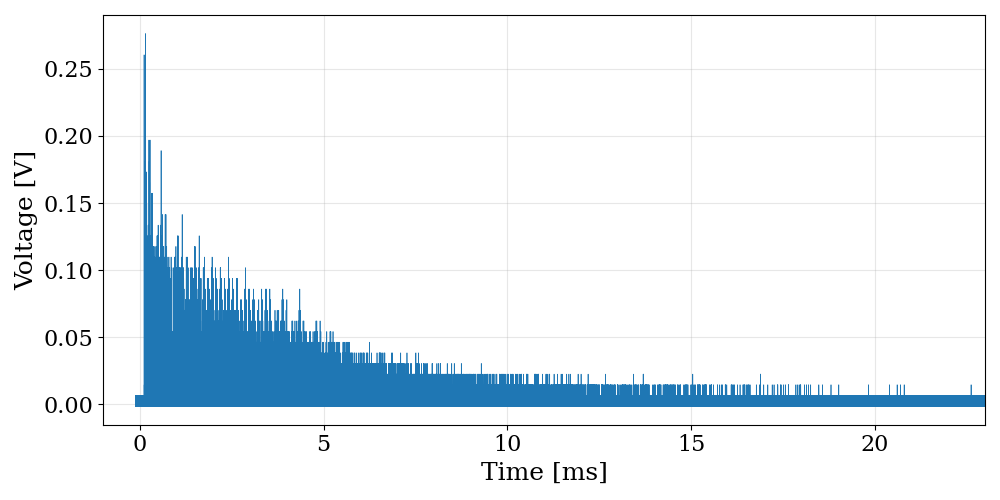
\includegraphics[width=0.8\columnwidth]{Figures/C04_Monitoring_system/waveform.png}
    \caption{Injection beam loss raw waveform}
    \label{fig:Injection beam loss raw waveform}
\end{figure}

\begin{figure}[htbp]
    \centering
    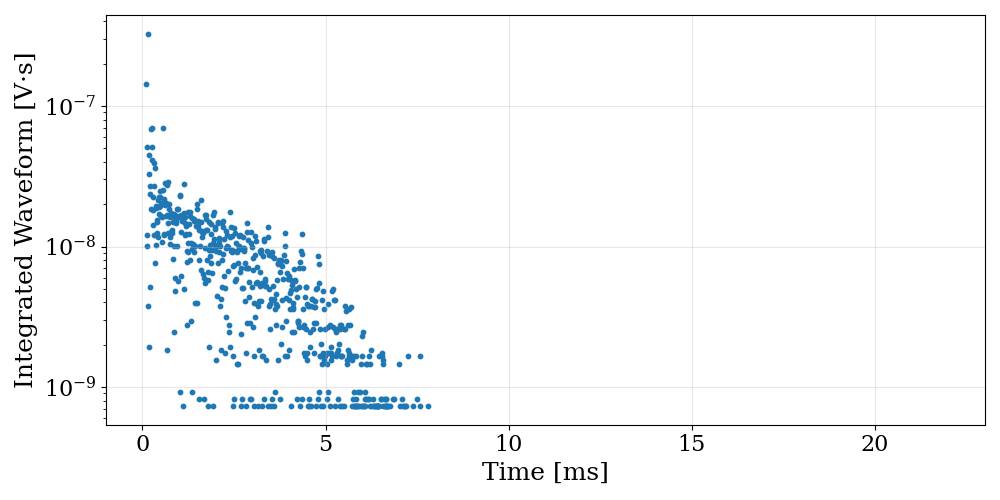
\includegraphics[width=0.8\columnwidth]{Figures/C04_Monitoring_system/pulseintegral.png}
    \caption{Integrated injection beam loss turn-by-turn}
    \label{fig:Integrated injection beam loss turn-by-turn}
\end{figure}

These quantities are recorded as process valuables (PVs) in the Archiver, the data archiving system used at SuperKEKB. This allows the data to be accessed by users.